\section{Outline}


% https://en.wikipedia.org/wiki/Scientific_method

\subsection{Formulation of a Question: Do HPC kv applications need dynamic load
balancing policies or is there a one-size-fits-all policy?}

\subsection{Hypothesis: The Mantle approach is an effective mechanism for
switching load balancing policies in HPC key-value applications}

\begin{itemize}
  \item Mantle is a load balancing approach and API.
  \begin{itemize}
    \item quantifies effect of load balancing
    \item formalized effective FS balancers
    \item debugging tool 
  \end{itemize}
  \item HXHIM has migration mechanisms for load balancing
  \begin{itemize}
    \item bulk operations (\texttt{put/get()})
    \item key partitioners
    \item secondary indices
  \end{itemize}
\end{itemize}

\subsection{Prediction}

In order from most likely to least likely:

\begin{enumerate}

  \item HPC key-value store workloads are structured (because they are mostly
  workflows and simulations) that their job phases can be learned and exploited
  using dynamic load balancing policies.

  \item HPC key-value store workloads are so structured that one
  policy-fits-all

  \item HPC key-value store workloads are not structured enough to be learned

  \item HPC key-value store workload hotspots/flash crowds are too fast to be
  exploited

\end{enumerate}

\subsection{Testing: Combine Mantle and HXHIM to explore dynamic load balancing
policies for ParSplice, an HPC application with distinct workload phases}

\subsubsection{ParSplice is structured}
Figure~\ref{fig:scale-length}.
\begin{figure*}[tbh]
  \noindent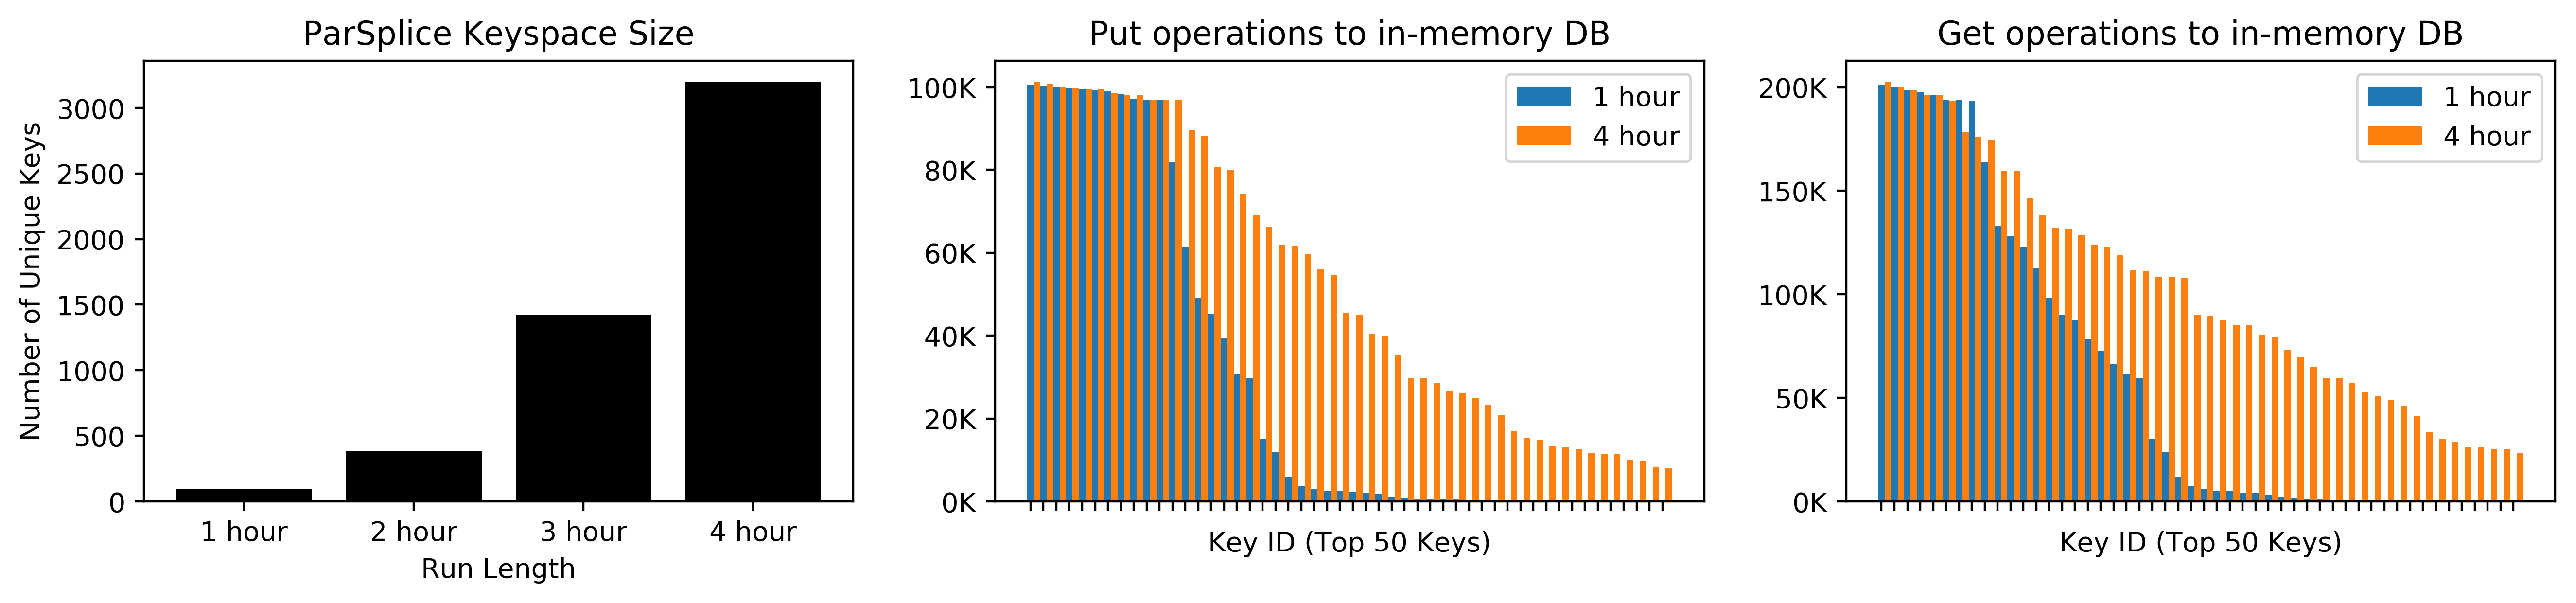
\includegraphics[width=1\textwidth]{figures/scale-length.png}\\
  \caption{We can predict how fast the keyspace grows and which parts of the
  namespace are popular.\label{fig:scale-length}}
\end{figure*}


\subsubsection{ParSplice behavior can change}

Figure~\ref{fig:scale-delay}.
\begin{figure}[tbh]
  \noindent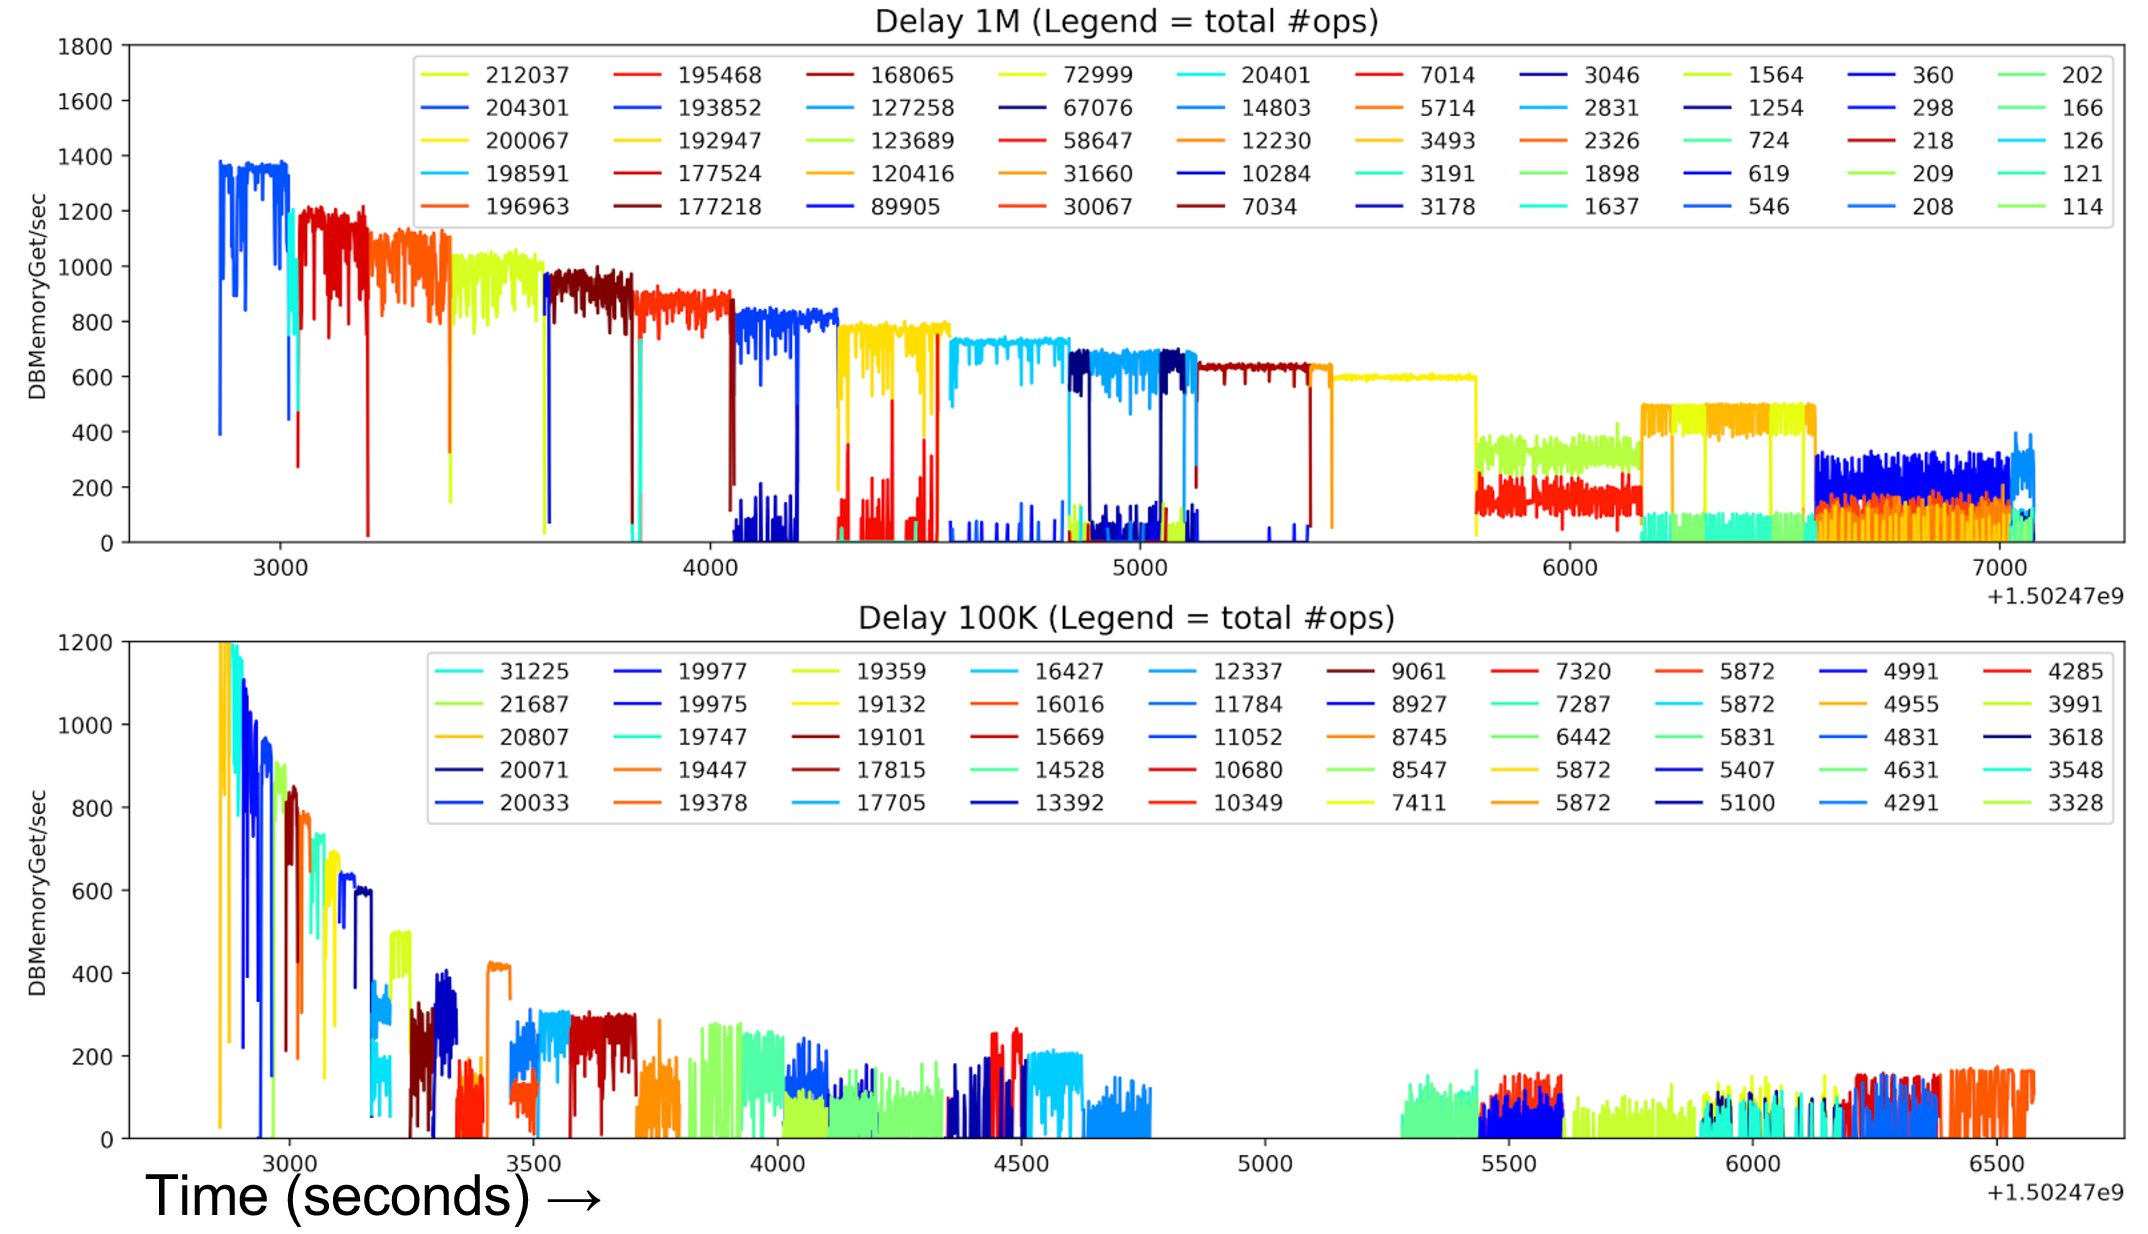
\includegraphics[width=0.5\textwidth]{figures/scale-delay.png}\\
  \caption{With a simple parameter tweak, the workload regimes changes
  (timescale) so one size does not fit all.  \label{fig:scale-delay}}
\end{figure}



\subsection{Analsyis}

\pagebreak
